\documentclass[a3paper, ngerman, 8pt]{article}

\usepackage[utf8]{inputenc}
\usepackage[margin=0.5cm, includefoot]{geometry}
\usepackage{multicol}
\usepackage{graphicx}
\usepackage[hidelinks]{hyperref}
\usepackage{fancyhdr}
\usepackage{lastpage}
\usepackage[ngerman]{babel}
\usepackage{titlesec}
\usepackage{calc}
\usepackage{enumitem}
\usepackage{amsmath}
\usepackage{amssymb}
\usepackage{ifthen}
\usepackage{color}
\usepackage{textcase}
\usepackage{capt-of}
\usepackage{listings}
\usepackage{framed}
\usepackage{dsfont}
\usepackage{tikz}
\usepackage{amsmath}

\usepackage{lipsum}	% für Dummy-Text

%
\hypersetup{
	unicode=true,
	pdftitle={Analysis},
	pdfauthor={Flavia Bindschedler, Mathias Graf},
	pdfsubject={Zusammenfassung Analysis},
	pdfcreator={LaTeX},
	pdfproducer={pdflatex},
	pdfnewwindow=true
}

% Abstand und Linienbreite zwischen Spalten
\setlength{\columnsep}{1cm}
\setlength{\columnseprule}{0.4pt}

% kein Einrücken bei neuem Absatz
\setlength{\parindent}{0pt}

% Weniger Abstand vor und nach überschriften
\titlespacing\section{0pt}{12pt plus 4pt minus 2pt}{0pt plus 2pt minus 2pt}
\titlespacing\subsection{0pt}{12pt plus 4pt minus 2pt}{0pt plus 2pt minus 2pt}
\titlespacing\subsubsection{0pt}{12pt plus 4pt minus 2pt}{0pt plus 2pt minus 2pt}

\pagestyle{fancy}

% Footer konfigurieren
\makeatletter
\lfoot{\@title}
\cfoot{\today}
\rfoot{Seite~\thepage~von~\pageref{LastPage}}
\makeatother
\renewcommand{\footrulewidth}{0.4pt}							% hrule über footer

\renewcommand{\labelitemi}{$\vcenter{\hbox{\tiny$\bullet$}}$}	% kleinere Dots in Itemize

\newcommand{\tipp}[1]{\vspace{-1.5em}\begin{framed}Tipp: \emph{#1}\end{framed}\vspace{-1.5em}}

\newcommand*\circled[1]{\tikz[baseline=(char.base)]{
		\node[shape=circle,draw,inner sep=1pt] (char) {#1};}}
\newcommand{\mbeq}{\overset{!}{=}}

% Titel und Author
\title{Zusammenfassung Analysis II}
\author{Flavia Bindschedler}
\def\email{\href{mailto:flavia.bindschedler@uzh.ch}{\texttt{flavia.bindschedler@uzh.ch}}}

\begin{document}

% Titel setzen
\makeatletter
{\Large \textbf{\@title}}
\hfill
{\@author}
\makeatother
\hrule

\begin{multicols*}{3}

\subsection*{Stetigkeit und Differenzierbarkeit:} Eine Funktion f ist an der Stelle $x_0$ diff'bar, falls: $ \lim_{h \to 0} \frac{f(x_0+h)-f(x_0)}{h}$ existiert. Diffbarkeit $\implies$ Stetigkeit

\textit{\textbf{Stetig, Diff'bar?} In der Regel ist es eine Komposition stetig diff'barer Funktionen und somit überall ausser in $x\neq ?$ stetig diff'bar. Für die Stetigkeit schauen wir uns den GW der Funktion von beiden Seiten an, muss gleich sein. Für die Differenzierbarkeit nehmen wie den Differnezenquotienten (siehe oben), von beiden Seiten gleich}

\textit{\textbf{Diff'barkeit in $\mathbb{R}^n$:} zuerst die partiellen Ableitungen berechnen, um zu zeigen, dass diese gleichzeitig existieren (wenn es eine aufgeteilte Funktion ist, dann den Teil um den kritischen Punkt nehmen). Das Differential ist: $df \vert _{{x_0, y_0}} (v) = \frac{\partial }{\partial x} (x_0, y_0)v_1 + \frac{\partial }{\partial y}(x_0, y_0)v_2$. Nun berechnen wir: $R(v)=f(v) - f(x_0, y_0) - df(v)$, wobei $v=(v_1, v_2)$. Der GW  $\lim_{v \to (x_0, y_0)} \frac{R(v)}{\vert v \vert} = 0$}

\textbf{Stetigkeit in $\mathbb{R}^n$:} Polarkoordinatentrick ist nützlich: $x= rcos\phi, y=rsin\phi$, falls der GW nur von $\phi$ abhängt, dann existiert der GW nicht. \textit{\textbf{in einem Punkt:} beide partielle Ableitungen berechnen, die GW der Abtleitungen nach gefragtem Punkt müssen gleich sein.}

\textbf{Lipschitz-Stetigkeit:} Eine Funktion ist Lipschitz stetig, fall die Ableitung beschränkt ist (geht in keinem Punkt gegen unendllich). Ist etwas nicht Lipschitz stetig, kann es gar nicht dem Satz von Picard-Lindelöf widersprechen. 


\textbf{Satz von Picard-Lindelöf:} Eine Funktion ist in der zweiten Variabel Lipschitz-stetig, also: $\exists L > 0$ mit $\vert \vert f(x,y)-f'(x,y')\vert \vert \leq L\vert \vert y-y'\vert \vert$. Dann gibt es ein $\epsilon > 0$ sodass das Anfangswertproblem 
$\begin{vmatrix}
	y'(x)=f(x,y)\\
	y(x_0)=y_0
\end{vmatrix}$ eine eindeutige Lösung hat $y\in C'([x_0-\epsilon, x_0+\epsilon], \mathbb{R}^n)$ $\to $ Eindeutigkeit (wir können sagen, dass wenn die Ableitung einer Funktion beschränkt ist, dann existiert in einem Intervall eine eindeutige Lösung)

\textbf{Satz von Schwarz:} ist eine Funktion 2x diff'bar und die 2ten Ableitungen sind stetig, dann kann man die partiellen Ableitungen vertauschen: $\frac{\partial ^2 f}{\partial x_i \partial x_j}= \frac{\partial ^2 f}{\partial x_j \partial x_i}$

\textbf{Hesse-Matrix:} $H_f=\begin{pmatrix}
\frac{\partial ^2 f}{\partial x_1^2} & ... &\frac{\partial ^2 f}{\partial x_1 \partial x_n} \\
...& ... & ... \\
\frac{\partial ^2 f}{\partial x_n \partial x_1} & ... & \frac{\partial ^2 f}{\partial x_n^2}
\end{pmatrix}$ 

ist diese Matrix indefinit $\leftrightarrow$ keine lokalen Extrema

\textbf{Maxima und Minima in $\mathbb{R}^n$:} zuerst bestimmen wir von f(x,y) den Gradienten und schauen bei welchen Werten für x und y die Einträge 0 sind. Anschliessend bestimmen wir die Hesse-Matrix, setzen die gefundenen Werte ein (wenn x gefunden, dann y berechnen). Wir berechnen die Determinante und die Werte für $\lambda$. \underline{positiv definit} $\to$ Minimum, \underline{negativ definit} $\to$ Maximum, \underline{indefinit} $\to$ Sattelpunkt, \underline{positiv semidefinit} $\to$ Minimum oder  Sattelpunkt, \underline{negativ semidefinit} $\to$ Maximum oder  Sattelpunkt

\textit{\textbf{Extrema mit Nebenbedingungen:} gegeben sind in der Regel f und eine Nebenbedingun aus der wir g = 0 finden (alles auf eine Seite). Dann machen wir ein Gleichungssystem:}

$\begin{vmatrix}
\partial_xf(x,y) = \lambda \partial_x g(x,y) \\
\partial_yf(x,y) = \lambda \partial_y g(x,y)\\
g(x)=0
\end{vmatrix}$

\textit{meistens gibt es einen trivialen Zusammenhang wie z.B. $-4x=2\lambda x$, dann untersucht man die Funktionen für $x=0$ und $x\neq 0$. Setzen die $x$ in f ein. Für $f(x)\leq 0 \to Minimum$}

\textbf{kritische Punkte:} für Gradient der Funktion = $0$

\textit{\textbf{Mannigfaltigkeit:} zeigen, dass etwas eine Mannigfaltigkeit der dim=2 ist: eine Funktion definierren, Differential davon nehmen = (0,0,0) $\to$ hat es kritische Punkte für die das erfüllt ist? wenn nicht $\in \mathbb{R}^n$ und somit dimension $k=n-1$}

\textbf{Differential:}

$Df=\begin{pmatrix}
\frac{\partial f_1}{\partial x_1} & ... & \frac{\partial f_1}{\partial x_n}\\
... & ...& ...\\
\frac{\partial f_m}{\partial x_1} & ... & \frac{\partial f_m}{\partial x_n}
\end{pmatrix}$


\subsection*{Differentialgleichungen}
\textbf{Trennung der Variabeln:} erst $y'=\frac{dy}{dx}$ umschreiben, alle x und alle y auf eine Seite. Integrieren und c nicht vergessen. Nach y auflösen, die Anfangsbedingungen einsetzen um c zu finden. in y(x) einsetzen und fertig. 

\textbf{Substitutionen:} 

\textit{Form:} $y'=h(\frac{y}{x})$ auf $\frac{y}{x}$ \textbf{achten}, dann $z=\frac{y(x)}{x}$ und $y'=z+xz'$ einsetzen und nach z lösen, dann Rücksubstitution. 

\textit{Form:} $y'=h(ax+by+c)$, substituieren: $z(x)=ax+by+c$, $y'=\frac{z'-a}{b}$ die Werte für a,b,c mit vergleichen finden. 

\textit{Form:} $y'=h(\frac{ax+bx+c}{dx+ey+f})$, Gleihcungssystem mit Zähler und Nenner = 0, $z=y-y_0$, $t=x-x_0$, $y'=z'$

\textit{Form:} $y'=\frac{x}{y}h(xy)$, $z=xy$, $y'=\frac{xz'-z}{x^2}$

\textit{Form:}$y'=h(x)y+g(x)y^a$, $z=y^{1-a}, y'=\frac{1}{1-a}z^{a/(1-a)z'}$

\textbf{Eindeutigkeit von Anfangswertproblemen:} Falls wie zeigen müssen, dass eine Funktion y definiert ist durch eine aufgeteilte Funktion müssen wir zeigen, dass die Funktion und die Ableitung stetig sind, also GW von oben und unten gleich. $\to$ Picard-Lindelöf


\subsection*{Produkt-, Quotienten-, Kettenregel} $(f\cdot g)'(x_0) = f(x)g'(x)+g'(x)f(x)$ $\big \vert$  $(\frac{f}{g})'(x_0) = \frac{g(x)f'(x)-f(x)g'(x)}{g^2(x)}$ $\big \vert$ $(g\circ f)'(x_0)=g'(f(x))\cdot f'(x)$ $\big \vert$ $[a^{u(x)}]'= ln(a)\cdot a^{u(x)}\cdot u'(x)$

\subsection*{Mittelwertsatz:} ist $f: [a,b]$ stetig, $f:(a,b)$ diff'bar $\exists f'(c)=\frac{f(b)-f(a)}{b-a}$ for a $c\in (a,b)$

\textit{\textbf{Anwendung Mittelwertsatz:} $|f(b)-f(a)|=f'(c)\cdot |b-a| \to |f(b)-f(a)|\leq M \cdot |b-a|$, wobei $|f'(x)|\leq M $, $x \in (a,b)$}

\textbf{Satz von Bernoulli de l'Hôpital:}

\textbf{Satz von Rolle:} $f: [a,b]$ stetig, $f:(a,b)$ diff'bar, $f(a)=f(b)$ $\exists c \in (a,b)$ s.d $f'(c)=0$

\subsection*{Konkav, Konvex:} konkav wenn $f''\geq0$, konvex $f''\leq 0$

\subsection*{Taylorpolynom}
$f(x)=f(a)+f'(a)(x-a)+...+\frac{1}{m!}f^{m}(a)(x-a)^m+\frac{1}{(m+1)!}f^{(m+1)}(c)(x-a)^{m+1}$

Alle bis zur m-ten Ableitungen berechnen und Punkt a einsetzen. Und dann einfach Formel (oben) anweden, m ist die Ableitung. 

$P(x)=\sum_{n=0}^{\infty}\frac{1}{n!}f^{(n)}(a)(x-a^n)$

\textbf{Taylorpolynom zweiter Ordnung in Punkt $(a_1, a_2, a_3)$:} $f(a) + \nabla f(a)\cdot h + \frac{1}{2}h^TH_f(a)h$ das entspricht: $f(a) + h_1 \frac{\partial f(a)}{\partial x}+h_2\frac{\partial f(a)}{\partial y}+h_3\frac{\partial f(a)}{\partial z}+\frac{1}{2}(h_1^2\frac{\partial^2 f(a)}{\partial x^2}+h_2^2\frac{\partial^2 f(a)}{\partial y^2}+h_3^2\frac{\partial^2 f(a)}{\partial z^2}+2h_1h_2\frac{\partial ^2 f}{\partial x \partial y}+2h_1h_3\frac{\partial ^2 f}{\partial x \partial z}+2h_2h_3\frac{\partial ^2 f}{\partial y \partial z})$, $h_1=(x-a_1)$, $h_2=(x-a_2)$, $h_1=(x-a_2)$

\textit{\textbf{n-tes Taylorpolynom der Funktion $f(x)$ um Punkt $a$ finden mit $x \in I$}}

\textbf{Bekannte Taylorreihen:} $\frac{1}{1-x}=1+x+x^2+...=\sum_{n=0}^{\infty}x^n$ $\to$ können in einem Bruch einfach $x$ ersetzen. $\big \vert$ $cos(x)=1-\frac{x^2}{2!}+...=\sum_{n=0}^{\infty}\frac{(-1)^n x^{2n}}{2n!}$

\textbf{Lagrange error bound, Fehlerterm:} $|R_n(x,a)| = |f(x)-p_n(x,a)|\leq \frac{max_{\xi \in [a,x]}|f^{{(n+1)}}(\xi)|}{(n+1)\!}|x-a|^{n+1}$

\textit{für die gegebene Funktion die n-te Ableitung aufschreiben, dann $[x, a]$ bestimmen, diese Variabeln und die Ableitung einsetzen, $\xi$ so wählen, dass das Maximum gegeben ist. Auch Variabeln für z.B. $a$ maximal wählen und Fehlerterm final aufschreiben}

\subsection*{Vektoranalysis}
\textbf{Richtungsableitung:} gegeben sind ein stetig diff'bares Skalarfeld $ f: \Omega \subset \mathbb{R}^n \to \mathbb{R}^n$ und ein Einheitsvektor $\vec{e}$. Die Richtungsableitung ist dann $D_{\vec{e}}f(x_0)\equiv\vec{e} \cdot \nabla f(x_0)$

\textit{\textbf{Richtungsableitungen von f an Stelle $(x_0,y_0)$ in eine bel. Richtung $v=(a,b)\neq (0,0)$} Wir schreiben zuerst das auf: $D_vf(x_0, y_0)=\lim_{h \to 0}\frac{f(x_0+ha, y_0+hb)-f(x_0, y_0)}{h}$} und bestimmen das/die Limits. Können mehrere sein, falls z.b a im Nenner ist $\to$ müssen dann den Fall $a=0$ extra berechnen. 

\textbf{Tagentialebene an $S=t_1+t_2+t_3$  in $\bar{x}$:} $T_{\bar{x}} = \{(x_1, x_2, x_3)\in \mathbb{R}^n (x-\bar{x})\cdot \nabla \Phi(\bar{x})=0\}$, also alle Ableitungen addiert mit $ (x-\bar{x}, y-\bar{y}, z-\bar{z})$ jeweils multipliziert. \textit{Wir suchen die \underline{Schnittpunkte $(t_1, t_2, t_3)$} der TE mit den Koordinatenachsen:wir setzen $(x=t_1, y=0, z=0)$ in die Menge von vorher ein, aber nur für das $x\in(x-\bar{x})$. Machen das gleiche für $y$ und $z$. }

\textbf{Flächen berechnen:} Wir haben eine Funktion in $\mathbb{R}^2$ und sollen den Flächeninhalt einer Menge in $\mathbb{R}^3$ berechnen. Meistens ist $z$ dann in dieser Menge gegeben (direkt oder indeirekt). Wir schreiben dann: $(x,y) \to (x,y,z)$, wobei in z irgendwas eingesetzt wird. Je nachdem machen wir Koordinatentransformation und müssen die Bedingungen gegeben in der Menge noch damit umschreiben. Wir leiten dann von $(x,y,z)$ jeweils nach nach Variabeln vom Anfanf $(x,y)$ ab und kriegen 2 Vektoren: $\phi_x$ und $\phi_y$ (\textbf{Tangentialvektoren}). Wir berechnen dann das Kreuzprodukt und nehmen den Betrag (Wurzel von Summe von Komponenten hoch 2). Mit diesem Betrag schreiben wir den Flächeninhalt: $\mu (F)= \int_{A} \vert \phi_x \times \phi_y \vert dxdy$. Integral berechnen (vlt vorher noch Transformation, und die umgeformten Bedingungen als Integrationsgrenzen) und finito.

\textbf{Vektorfeld:} ist eine Abb. $\mathbb{R}^n \to \mathbb{R}^m$, welche jedem Punkt x des Definitionsbereichs einen Vektor mit m Komponenten zuordnet. $x \to \begin{pmatrix}
v_1(x_1, ..., x_n) \\
...\\
v_m(x_1, ... x_n)
\end{pmatrix}$

\textbf{Feldlinien: } K ist ein Vektorfeld. Eine parametrisierte Kurve heisst Feldlinie, falss $\gamma ' (t)$ für alle $t\in I \propto K(\gamma (t))$. Eine natürliche Feldlinie ist durch $\gamma ' (t) = K(\gamma (t))$ bestimmt! (können also eine Zahl $L$ als Proportionalitätskonstante wählen $\to L\gamma ' (t) = K(\gamma (t))$) 

Können das benutzen um ein Vektorfeld zu konstruieren.

\textbf{Gradien:} $\begin{pmatrix}
\frac{\partial f}{\partial_{x_1}} \\
... \\
\frac{\partial f}{\partial_{x_n}}
\end{pmatrix}$, zeigt Richtung der max. Zuwachsrate.

\textbf{Gradientfelder:} \fbox{$K=\nabla \phi$}, \fbox{$K_x = \frac{\partial \phi}{\partial x}$}
 Damit ein Vektorfeld ein Gradienfeld ist muss man zeigen: $\frac{\partial K_x}{\partial y}$ = $\frac{\partial K_y}{\partial x}$ (also erste Komponente nach y und zweite nach x ableiten). Um das \textbf{Potentialfeld} zu bestimmen, findet man: 

$\phi(x,y) = \int K_x dx + \psi(y)$ 

$\psi(y)=\int K_y dy + c$

Wir setzen alles in $\phi(x,y)$ ein und haben das Potentialfeld gefunden. Überprüfen, dass $K_y\neq\frac{\partial \phi}{\partial y}$, sonst entfällt die Ableitung $\frac{\partial \psi}{\partial y}$ und wir haben nur die erste Gleichung mit Konstante c dann. 

\textbf{Gradientfeld mit 3 Variabeln:} es muss gelten:

$\frac{\partial K_z}{\partial y}-\frac{\partial K_y}{\partial z} = 0$, $\frac{\partial K_x}{\partial z}-\frac{\partial K_z}{\partial x} = 0$, $\frac{\partial K_y}{\partial x}-\frac{\partial K_x}{\partial y} = 0$,

\textbf{Potential $\phi$ finden:} $\begin{pmatrix}
K_1 \\ K_2 \\ K_3 
\end{pmatrix}$ = 
$\begin{pmatrix}
\frac{\partial \phi}{\partial x} \\ \frac{\partial \phi}{\partial y} \\ \frac{\partial \phi}{\partial z} 
\end{pmatrix}$, wobei K gegeben

Wir fangen mit einer Gleichung an: $\frac{\partial\phi}{\partial x}\mbeq K_1 \to \phi = \int K_1 dx = $ etwas $+C(y,z)$, dann diese Lösung in eine zweite einsetzen: $\frac{\partial\phi}{\partial y}=\frac{etwas + c(y,z)}{\partial y}= $smth$ + \frac{\partial c(y,z)}{\partial y} \mbeq K_2 $

$\to \frac{\partial c(y,z)}{\partial y} =$ smthelse, wir integrieren: $c=$ etwas + Etwas + D(z). Wir setzen das in unser erstes $\phi$ ein und kriegen: $\phi =$ etwas + Etwas + D(z). Das setzen wie in die anderen 2 partiellen Ableitungen ein und finden D(z) (dazu vergleichen wir mit den partiellen Ableitungen von K, denn $K=\nabla \phi$ und passen mithilfe von D so an, dass es mit den Ableitungen übereinstimmt). Arbeit: $\phi (B)-\phi(A)$


\textbf{Divergenz:} $div(\vec{v})=\nabla \cdot \vec{v}=\frac{\partial v_1}{\partial x_1}+...+\frac{\partial v_n}{\partial x_n}$

\textbf{Satz von Gauss:} \fbox{$\int_{\partial \Sigma}\vec{V}\cdot \vec{n} d \Omega= \int_{\Sigma}\vec{\nabla}\cdot\vec{v}d\mu$} von Fluss durch \textbf{Fläche} nach \textbf{Volumen}. $/vec{V}$ ist ein Vektorfeld, $\Sigma$ ein glatt berandeter Bereich.

\subsection*{Riemann'sche Summe}
\textbf{Obersumme:} $\bar{S}=\sum_{i=1}^{n} \Delta x \cdot \Delta y$, wobei $\Delta x = \frac{Intervall}{n}$, also z.B für ein Interval $[0,2] \to \Delta x = \frac{2}{n}$. Und: $\Delta y = f(\Delta x \cdot i)$.
\textit{Können alles ausser die $i$ abhängigen Terme vor das Summenzeichen nehmen und in mehrere Summen aufteilen. Für Funktionen mit x und y, einfach gelich machen, aber dann um $\Delta y$ zu finden $x=\Delta x$ einsetzen.}

\textbf{Untersumme:} $\underline{S}=\sum_{i=1}^{n} \Delta x \cdot \Delta y$, wobei $\Delta x = \frac{Intervall}{n}$ und: $\Delta y = f(\Delta x \cdot (i-1))$

\fbox{für $n\to \infty$:  $\bar{S}=\underline{S}$ $\to$ integrierbar mit diesem GW}

\textbf{bekannte Summen:} $\sum_{i=1}^{n} i^2 = \frac{n(n+1)(2n+1)}{6}$ $\big \vert$ $\sum_{i=1}^{n} i = \frac{n(n+1)}{2}$  $\big \vert$ $\sum_{i=1}^{n} 1=n$ $\big \vert$ 

\subsection*{Integral}

\textbf{Linienintegrale:} Aufgabe: Berechnen Sie das Linienintegral $\int_{\gamma} Kdx$. K ist gegeben. Als erstes müssen wie $\gamma (t)$ aufschreiben (Z.B Plarkoordinaten für Einheitskreis, oder gegeben durch eine Gleichung). Dann berechnen wir $K(\gamma (t))$ und $\gamma ' (t)$. Dann integrieren wir: $\int_{\gamma} K(\gamma (t))\cdot \gamma ' (t)dt$, wobei die Grenzen durch Aufgabe oder Transformation gegeben sind (Skizze hilft).

\textit{\textbf{Partialbruchzerlegung falls Polynom im Nenner:} 1. Den Nenner faktorisieren 2. Nullstellen ablesen 3. Die Zerlegung aufschreiben und mit Nenner multiplizieren 4. Jede Nullstelle einsetzen, um A,B,... zu finden. 5. Diese einsetzen und Teile einzeln integrieren}
\textbf{Beispiel: }$f(x)=\frac{2x+3}{x^2-9}$, 1. $(x-3)(x+3)$ 2. 0-Stellen: $3, -3$ 3. $\frac{2x+3}{(x+3)(x-3)}=\frac{A}{x+3}+ \frac{B}{x-3} \to 2x+3=A(x-3)+B(x+3)$ 4. $A=\frac{1}{2}, B=\frac{2}{3}$ 5. $\int\frac{2x+3}{(x+3)(x-3)}dx=\int\frac{1}{2}\frac{1}{x+3}dx+ \int\frac{2}{3}\frac{1}{x-3}dx$

\textbf{Leibniz integral rule:} 

$\frac{\partial}{\partial x}\int_{\phi (x)}^{\Psi (x)}f(x,t)dt= f(x, \Psi(x))\Psi'(x)-f(x, \phi (x))\phi'(x)+\int_{\phi (x)}^{\Psi(x)}f'(x, t)$, die Integrationsgrenzen sind die Funktionen vor einer Funktion mit 2 Variabeln

\textbf{Patielle Integration:} $\int u dv=u\cdot v -\int v du$, \textbf{dv}: 1, falls $arc$ oder $log$, $x^n, \frac{1}{1\pm x^2}$
\textbf{u:}$x^n, log, arc, cos^n... $

\textbf{$x^2 + bla$ im Nenner:} $\int \frac{1}{8(x^2+4)}$ substituieren mit $x=2u \to u=\frac{x}{2}, du = \frac{1}{2}dx$ dann Integral: $\frac{1}{8}\int \frac{2}{4u^2+4}du \to \frac{1}{16} \int \frac{1}{u^2+4}du= \frac{arctan(u)}{16}$

\textbf{uneigentliche Integrale, Integral konvergent?:} einfach Integral berechnen und schauen, ob es einen Wert hat $\to$ konvergent, sonst divergent

\textbf{Satz von Fubini:} Sei Quader $Q=[a_1, b_1]\times[a_2, b_2]$ und $f: Q \to \mathbb{R}^n$ mit $f \in C^0(\bar{Q})$, dann gilt: $\int_Q f(x,y)d\mu (x, y)= \int_{a_1}^{b_1}dx\int_{a_2}^{b_2}dy f(x,y)$ Integrationsreihenfolge ist frei wählbar. (Satz nur anwendbar für überall diff'bare Funktionen)

\textit{\textbf{Anwendung Satz von Fubini:} Meist sind Grenzen für x und y gegeben, was die Integrationsgrenzen werden. Wenn wir substituieren, um das Integral zu lösen, müssen wir diese Grenzen ändern. Also wenn z.B. $x\in [0,1]$ war, und wir neu nach dz integrieren wollen, dann setzen \textbf{wir x=1 in die Substitution ein} (vlt beide Grezen anpassen, auch bei 0!). Z.B. haben wir $z=\frac{xy}{2}$ definiert, dann ist die obere Integrationsgrenze: $\frac{y}{2}$. \textbf{Wenn eine Variabel in der Grenze vorkommt, müssen wie darauf achten, dass das die zweite Integration wird (dzdy). }}

Vielleicht wird auch ein Dreieck oder so gegeben, dann einfach einen Ausdruck für $x$ durch Steigung finden. 

\textbf{Integrale:} $\int ln(x)=x\cdot ln(x) - x + C$ $\big \vert$ $\int cos^2(x)=\frac{cos(x)\cdot sin(x) + x}{2}$ $\big \vert$ $\int cos^n(x)dx=\frac{n-1}{n}\int cos^{n-2}dx+\frac{cos^{n-1}(x)sin(x)}{n}$, für sinus einfach tauschen und minus!

\subsection*{Koordinatentransformation}
im Allgemeinen ist die Determinante des Differentials = Jacobi. 
\textbf{Polarkoordinaten: } $x= rcos\phi, y=rsin\phi$, Jacobi $=rdrd\phi$, 
\textbf{Elliptisch:} $x=racos\phi, y = rbsin\phi$, Jacobi $=abrdrd\phi$, \textbf{Zylinder:} $x=rcos\phi, y=rsin\phi, z=z$, Jacobi $=rdrd\phi dz$, \textbf{Kugel:} $x=rsin\theta cos\phi, y=rsin\theta sin\phi, z=rcos\theta$, Jacobi $=r^2sin\theta drd\theta d\phi$, $\theta \in (0,\pi), \phi \in [0,2\pi)$

\subsection*{Rechenregeln und random züügs:} 
\begin{itemize}
	\item wenn eine Fkt. symmetrisch ist, kann man einfach den positiven Definitionsbereich anschauen
	\item wenn ein Term bei ungeradem n -/+ $\to (-1)^{(n+1)/2}$, bei geraden $\to (-1)^{n/2}$ $ \big \vert$ für +/- $n \to n+2$
	\item $tanx = \frac{sinx}{cosx}$
	\item $sin^3=(1-cos^2)sin$
	\item $a \times b \times c = b(a \cdot c) + c(a \cdot b)$
	\item $ln(1)=0$

\end{itemize}

$\frac{d}{dx} |x| = \frac{x}{|x|}$ $\big \vert$ $\frac{d}{dx} \arcsin = \frac{1}{\sqrt{1-x^2}}$ $\big \vert$ $\frac{d}{dx} \arccos = -\frac{1}{\sqrt{1-x^2}}$ $\big \vert$ $\frac{d}{dx} \arctan = \frac{1}{1+x^2}$ $\big \vert$ $\frac{d}{dx} ln^2x = \frac{2lnx}{x}$ $\big \vert$ $\frac{d}{dx}cos^5x=-5cos^4xsinx$

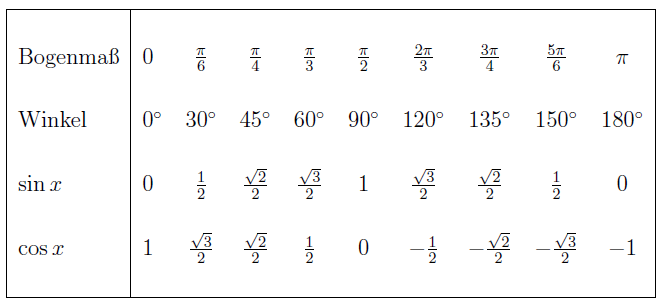
\includegraphics[width=1\linewidth]{winkel.png}





\end{multicols*}

\end{document}
